\NeedsTeXFormat{LaTeX2e}
\documentclass[a4paper,12pt,
headsepline,           % Linie zw. Kopfzeile und Text
oneside,               % einseitig
pointlessnumbers,      % keine Punkte nach den letzten Ziffern in Überschriften
bibtotoc,              % LV im IV
%DIV=15,               % Satzspiegel auf 15er Raster, schmalere Ränder   
BCOR15mm               % Bindekorrektur
]{scrbook}
\KOMAoptions{DIV=last} % Neuberechnung Satzspiegel nach Laden von Paket helvet

\pagestyle{headings}
\usepackage{blindtext}

% für Texte in deutscher Sprache
\usepackage[english]{babel}
\usepackage[utf8]{inputenc}
\usepackage[T1]{fontenc}

% Helvetica als Standard-Dokumentschrift
\usepackage[scaled]{helvet}
\renewcommand{\familydefault}{\sfdefault} 

% Literaturverzeichnis mit BibLKaTeX
\usepackage[babel]{csquotes}
\usepackage[backend=bibtex8,sorting=none,style=numeric-comp]{biblatex}
\bibliography{bibliography-prj}
\renewcommand*{\bibfont}{\small}

\usepackage{tikz}
\tikzset{every picture/.style={line width=0.75pt}} 

\usepackage{graphicx}
\usepackage{tabularx}
\usepackage{booktabs}
\usepackage{siunitx}
\usepackage{longtable}
\usepackage{multirow}
\usepackage{multicol}
\usepackage{float}
\usepackage{subfig}
\usepackage{dblfloatfix}

% Besondere Schriftauszeichnungen
\usepackage{xurl}              % \url{http://...} in Schreibmaschinenschrift
\usepackage{color}            % zum Setzen farbigen Textes
\usepackage{xcolor}
\usepackage{nicefrac}
\usepackage{amssymb, amsmath, amsthm} % Pakete für Mathe-Umgebungen und -Symbole

\newtheorem{definition}{Definition}

\usepackage{setspace}         % Paket für div. Abstände, z.B. ZA
\setlength{\parindent}{0pt}   % kein linker Einzug der ersten Absatzzeile
\setlength{\parskip}{1.4ex plus 0.35ex minus 0.3ex} % Absatzabstand, leicht variabel

% Tiefe, bis zu der Überschriften in das Inhaltsverzeichnis kommen
\setcounter{tocdepth}{3}      % ist Standard

% Beispiele für Quellcode
\usepackage{listings}
\definecolor{codegreen}{rgb}{0,0.6,0}
\definecolor{codegray}{rgb}{0.5,0.5,0.5}
\definecolor{codepurple}{rgb}{0.58,0,0.82}
\definecolor{backcolour}{rgb}{0.95,0.95,0.92}
\lstset{
	backgroundcolor=\color{backcolour},   
	commentstyle=\color{codegreen},
	keywordstyle=\color{magenta},
	numberstyle=\tiny\color{codegray},
	stringstyle=\color{codepurple},
	basicstyle=\ttfamily\footnotesize,
	breakatwhitespace=false,         
	breaklines=true,                 
	captionpos=b,                    
	keepspaces=true,                 
	numbers=left,                    
	numbersep=5pt,                  
	showspaces=false,                
	showstringspaces=false,
	showtabs=false,                  
	tabsize=2
}
\renewcommand{\lstlistingname}{Source Code}

\usepackage{booktabs}

% hier Namen etc. einsetzen
\newcommand{\fullname}{Jonathan Schilling}
\newcommand{\email}{jonathan.schilling@uni-ulm.de}
\newcommand{\titel}{Analysis of gameplay from the video game Valorant} 
\newcommand{\jahr}{2023}
\newcommand{\matnr}{980556}
\newcommand{\gutachterA}{Prof.\,Dr.\,Friedhelm Schwenker}
\newcommand{\betreuerB}{}
\newcommand{\betreuerA}{}
% hier die Fakultät auswählen
\newcommand{\fakultaet}{Engineering, Computer Science und Psychology}
% hier das Institut einsetzen
\newcommand{\institut}{Institute of Neural Information Processing}

% Informationen, die LaTeX in die PDF-Datei schreibt
\pdfinfo{
  /Author (\fullname)
  /Title (\titel)
  /Producer     (pdfeTex 3.14159-1.30.6-2.2)
  /Keywords ()
}

\definecolor{dark blue}{HTML}{000066}

\definecolor{todoCite}{HTML}{ABD4B6}%Quellen raussuchen
\definecolor{todoRef}{HTML}{A7C5DB}%Auf glossar, acronyme, bilder etc referenzieren
\definecolor{todoNorm}{HTML}{E6C59E}%Sonstige Todos
\definecolor{todoCont}{HTML}{B483C9}%Inhalte

\usepackage[hyperfootnotes=false]{hyperref}
\usepackage[multiple]{footmisc}
\usepackage[all]{hypcap}
\hypersetup{
pdftitle=\titel,
pdfauthor=\fullname,
pdfsubject={Project Thesis},
pdfproducer={pdfeTex 3.14159-1.30.6-2.2},
colorlinks=false,
linkcolor=dark blue,
citecolor=dark blue,
pdfborder=0 0 0	% keine Box um die Links!
}

\usepackage[toc,nonumberlist,nopostdot,nomain,acronym]{glossaries}\makeglossaries
%\newacronym[longplural={}]{acr-label}{short}{long}

\newacronym[description=Application Programming Interface]{acr-api}{API}{application 
programming interface}
\newacronym[name=mAP]{acr-mAP}{$mAP$}{Mean Average Precision}
\newacronym{acr-iou}{IoU}{Intersection over Union}
\newacronym[description=Convolutional Neural Network]{acr-cnn}{CNN}{convolutional neural 
network}
\newacronym[description=Feature Pyramid Network]{acr-fpn}{FPN}{feature pyramid network}
\newacronym[description=Non-maximum Suppression]{acr-nms}{NMS}{non-maximum suppression}
\newacronym[description=Batch Normalization]{acr-bn}{BN}{batch normalization}
\newacronym[description=Sigmoid Linear Unit]{acr-silu}{SiLU}{sigmoid linear unit}
\newacronym[description=Spatial Pyramid Pooling Fast]{acr-sppf}{SPPF}{spatial pyramid pooling 
fast}


% Trennungsregeln
\hyphenation{Hy-phe-na-tion}

\begin{document}
\frontmatter

% Titelseite
\thispagestyle{empty}
\begin{addmargin*}[4mm]{-1mm}
	
	\includegraphics[height=1.8cm]{images/unilogo_bild}
	\hfill
	\includegraphics[height=1.8cm]{images/unilogo_wort}\\[1em]
	
	{\footnotesize
		%{\bfseries Universität Ulm} \textbar ~89069 Ulm \textbar ~Germany
		\hspace*{99mm}\parbox[t]{44mm}{\bfseries Faculty of \fakultaet\\
			\mdseries \institut}\\[2cm]
		
		\parbox{143mm}{\bfseries \LARGE \titel}\\[2.5em]
		{\footnotesize Project Report at Ulm University}\\[3em]
		
		{\footnotesize \bfseries Submitted by:}\\
		{\footnotesize \fullname\\ \email}\\ \matnr\\[2em]
		{\footnotesize \bfseries Examiner:}\\                     
		{\footnotesize \gutachterA}\\[2em]
%		{\footnotesize \bfseries Betreuer:}\\ 
%		{\footnotesize \betreuerA\\ \betreuerB}\\\\
		{\footnotesize \jahr}
	}
\end{addmargin*}


% Impressum
\clearpage
\thispagestyle{empty}
{ \small
	\flushleft
	Edition: \today \\\vfill
	\copyright~\jahr~\fullname
}
% ab hier Zeilenabstand etwas größer 
\setstretch{1.2}

\tableofcontents

\mainmatter
\chapter{Introduction}\label{chpt:introduction}
\glsresetall

E-Sports is a growing market for years. The events become more professional, prize money is rising 
and even broadcasters like ProSieben MAXX already show such events on 
television~\cite{kovacevic}. In light of this, the performance pressure of teams get bigger and 
preparation effort increases. But what exactly is e-sports? The German Games Industry Association 
defines the term e-sports as a competition between two or more people playing video games 
according to fixed rules~\cite{kovacevic}. Those people are mostly organized in professional teams 
from all around the world. Common game genre for e-sports events are real-time strategy games, 
multiplayer online battle arena games, tactical shooters and sport simulations. For popular games 
like League of Legends (Riot Games), Counter Strike: Global Offensive (Valve) or FIFA (Electronic 
Arts)  various leagues and tournaments were founded and the players have to show their best 
performances to keep their place in the team as professional gamer. During the corona pandemic 
online content streaming on platforms like Twitch or Mixer became very popular and also the 
popularity of e-sports was boosted, which often is streamed on such platforms~\cite{kovacevic}. In 
that time a new tactic shooter was published: Valorant from Riot Games~\cite{riotgames-valorant}. It 
became a big hype and therefore the player base grew very fast, so that Riot Games decided to start 
a tournament the "Valorant Champions Tour" also called VCT~\cite{riotgames-vct}. A concept and 
first implementation for a tool that can help Valorant teams and players to improve their performance 
in e.g. the highly competitive VCT is introduced in this project report.

\section{Problem Definition}\label{sec:intro:problem}

After that short introduction to e-sports in general, the following section defines the problem that is 
addressed within that project. The initial idea of that project came from a Youtube 
video~\cite{river2021} in that someone tried to implement an artificial intelligent agent that plays the 
video game Valorant autonomously.
Such agents in general are a big problem in the gaming scene because some players try to gain an 
unfair advantage from 3rd party programs. Those programs are used to display more information for 
the players than intended or helps them to react faster and more precise on occurring events than it 
is possible for a human being. Due to that problem it is prohibited in the terms and conditions of 
online multiplayer games to use any type of additional programs to play the game. Furthermore there 
are anti-cheat mechanisms running on the same computer as the game, searching for suspect 
programs that try to manipulate the outcome of a match. If a cheat program is detected the player 
becomes banned from the game. Because of that fact it is not that easy to implement and test an 
artificial agent that plays the game.

Due to cheating concerns the video and its content could be condemned but the creator just had 
educational purposes, did not harmed any player and in the end the implemented agent would not be 
good enough to compete with average Valorant players. In the video the creator found a way that he 
could implement an agent that cannot be detected by the anti-cheat mechanisms: he placed the 
agent on a separate computer than the game. Additionally in difference to programs that try to 
cheat, the artificial agent only became the ability to interact with the game client as every human 
player. Input was the content of the in-game screen, captured completely legal and output of the 
agent were mouse and keyboard commands, that were transmitted to the computer with the 
Valorant client running. With that setup he successfully created a system that was able to play the 
game on a very basic level. Due to the reason that he showed a way that could make it possible to 
build a cheat-client that cannot be detected by the anti-cheat of Valorant he decided not to share 
his source code~\cite{river2021}.

So the first idea of the project was to recreate a similar agent, but that would have been too much 
for a single project. Therefore the next idea was to build an application that is able to 
analyze Valorant gameplay and helps to evaluate already played games for training purposes, as it is 
common in most ordinary sport disciplines. The task of that application is to generate alternative 
representations of game data. Normally data from matches is available as recorded video from 
player respectively observer view or as raw data saved in databases from the game publisher. A 
transformation of those data can result in a better overview and understanding of the whole match 
and what happens there. In a first step those generated transformations can be analyzed by a trainer 
or the players themselves. Later it would be possible to use this data again as input for other pattern 
recognition algorithms that try to find problems in rounds that were lost and flaws in the tactics of 
opponents or even to invent new tactics. Further it could be possible to train an artificial agent with 
such transformations as input and try to reach a new level of tactical understanding.

As already mentioned one possibility to get game data are databases from the game publisher. 
There is also an \gls{acr-api} that would provide all data from matches but it is impossible to get an 
\gls{acr-api}-Key if it is not used for an already publicly running and from Riot Games legitimated 
application. For this reason the raw data will be gameplay videos that become transformed into a 
simpler form of presentation.

Summarized the task of that project is to use a pattern recognition algorithm to transform a 
gameplay video of the computer game Valorant into a more compact and easier to understand data 
representation. That includes acquisition and pre-processing of data; selection, training and 
evaluation of a neural network; choosing a trained version for inference and preparation of the 
output data for presentation.

\section{Valorant}\label{sec:intro:valorant}

Valorant is a character-based tactical shooter from the publisher Riot Games, Inc. an American 
video game developer based in Los Angeles, California. In that game two teams consisting of 
respectively five players are competing against each other, trying to win rounds. The first team 
winning 13 rounds wins the whole match. The game is played on different maps, that are modeling
fictitious towns. In the context of this project the maps "Ascent", "Haven" and "Split" are relevant, 
but in total there are currently ten maps. At the start of the game each player of a team chooses one 
out of 22 agents whereby every agent only can be chosen once per team. Those agents are 
categorized by four character classes: Duelist, Initiator, Sentinels and Controllers. The tactical 
meaning of that classes is not important for this project. Which team begins on attacker side and 
which starts as defender is decided randomly. After twelve rounds the sides are switching. The goal 
of the attacking team is to place a bomb (also called Spike) on certain areas on the map or to kill the 
defending team. For that the attackers have 100 seconds, otherwise the defenders win the round. Is 
the Spike planted a countdown of 45 seconds starts until detonation. In that time the defending team 
has the possibility to defuse the bomb and win the round for themselves. When the Spike explodes 
after the 45 seconds the attackers are winning the round. The last option for the defenders to win a 
round is to kill the whole attacking team and avoid that the bomb explodes if it was planted. To win a 
round each player can choose from a variety of weapons like in all shooter games. One special 
feature of Valorant is that every agent has a distinct set of abilities. Those abilities bring additional 
options to make an impact on the round~\cite{riotgames-valorant, spike2023, unrated2023}.

\begin{figure}
	\centering
	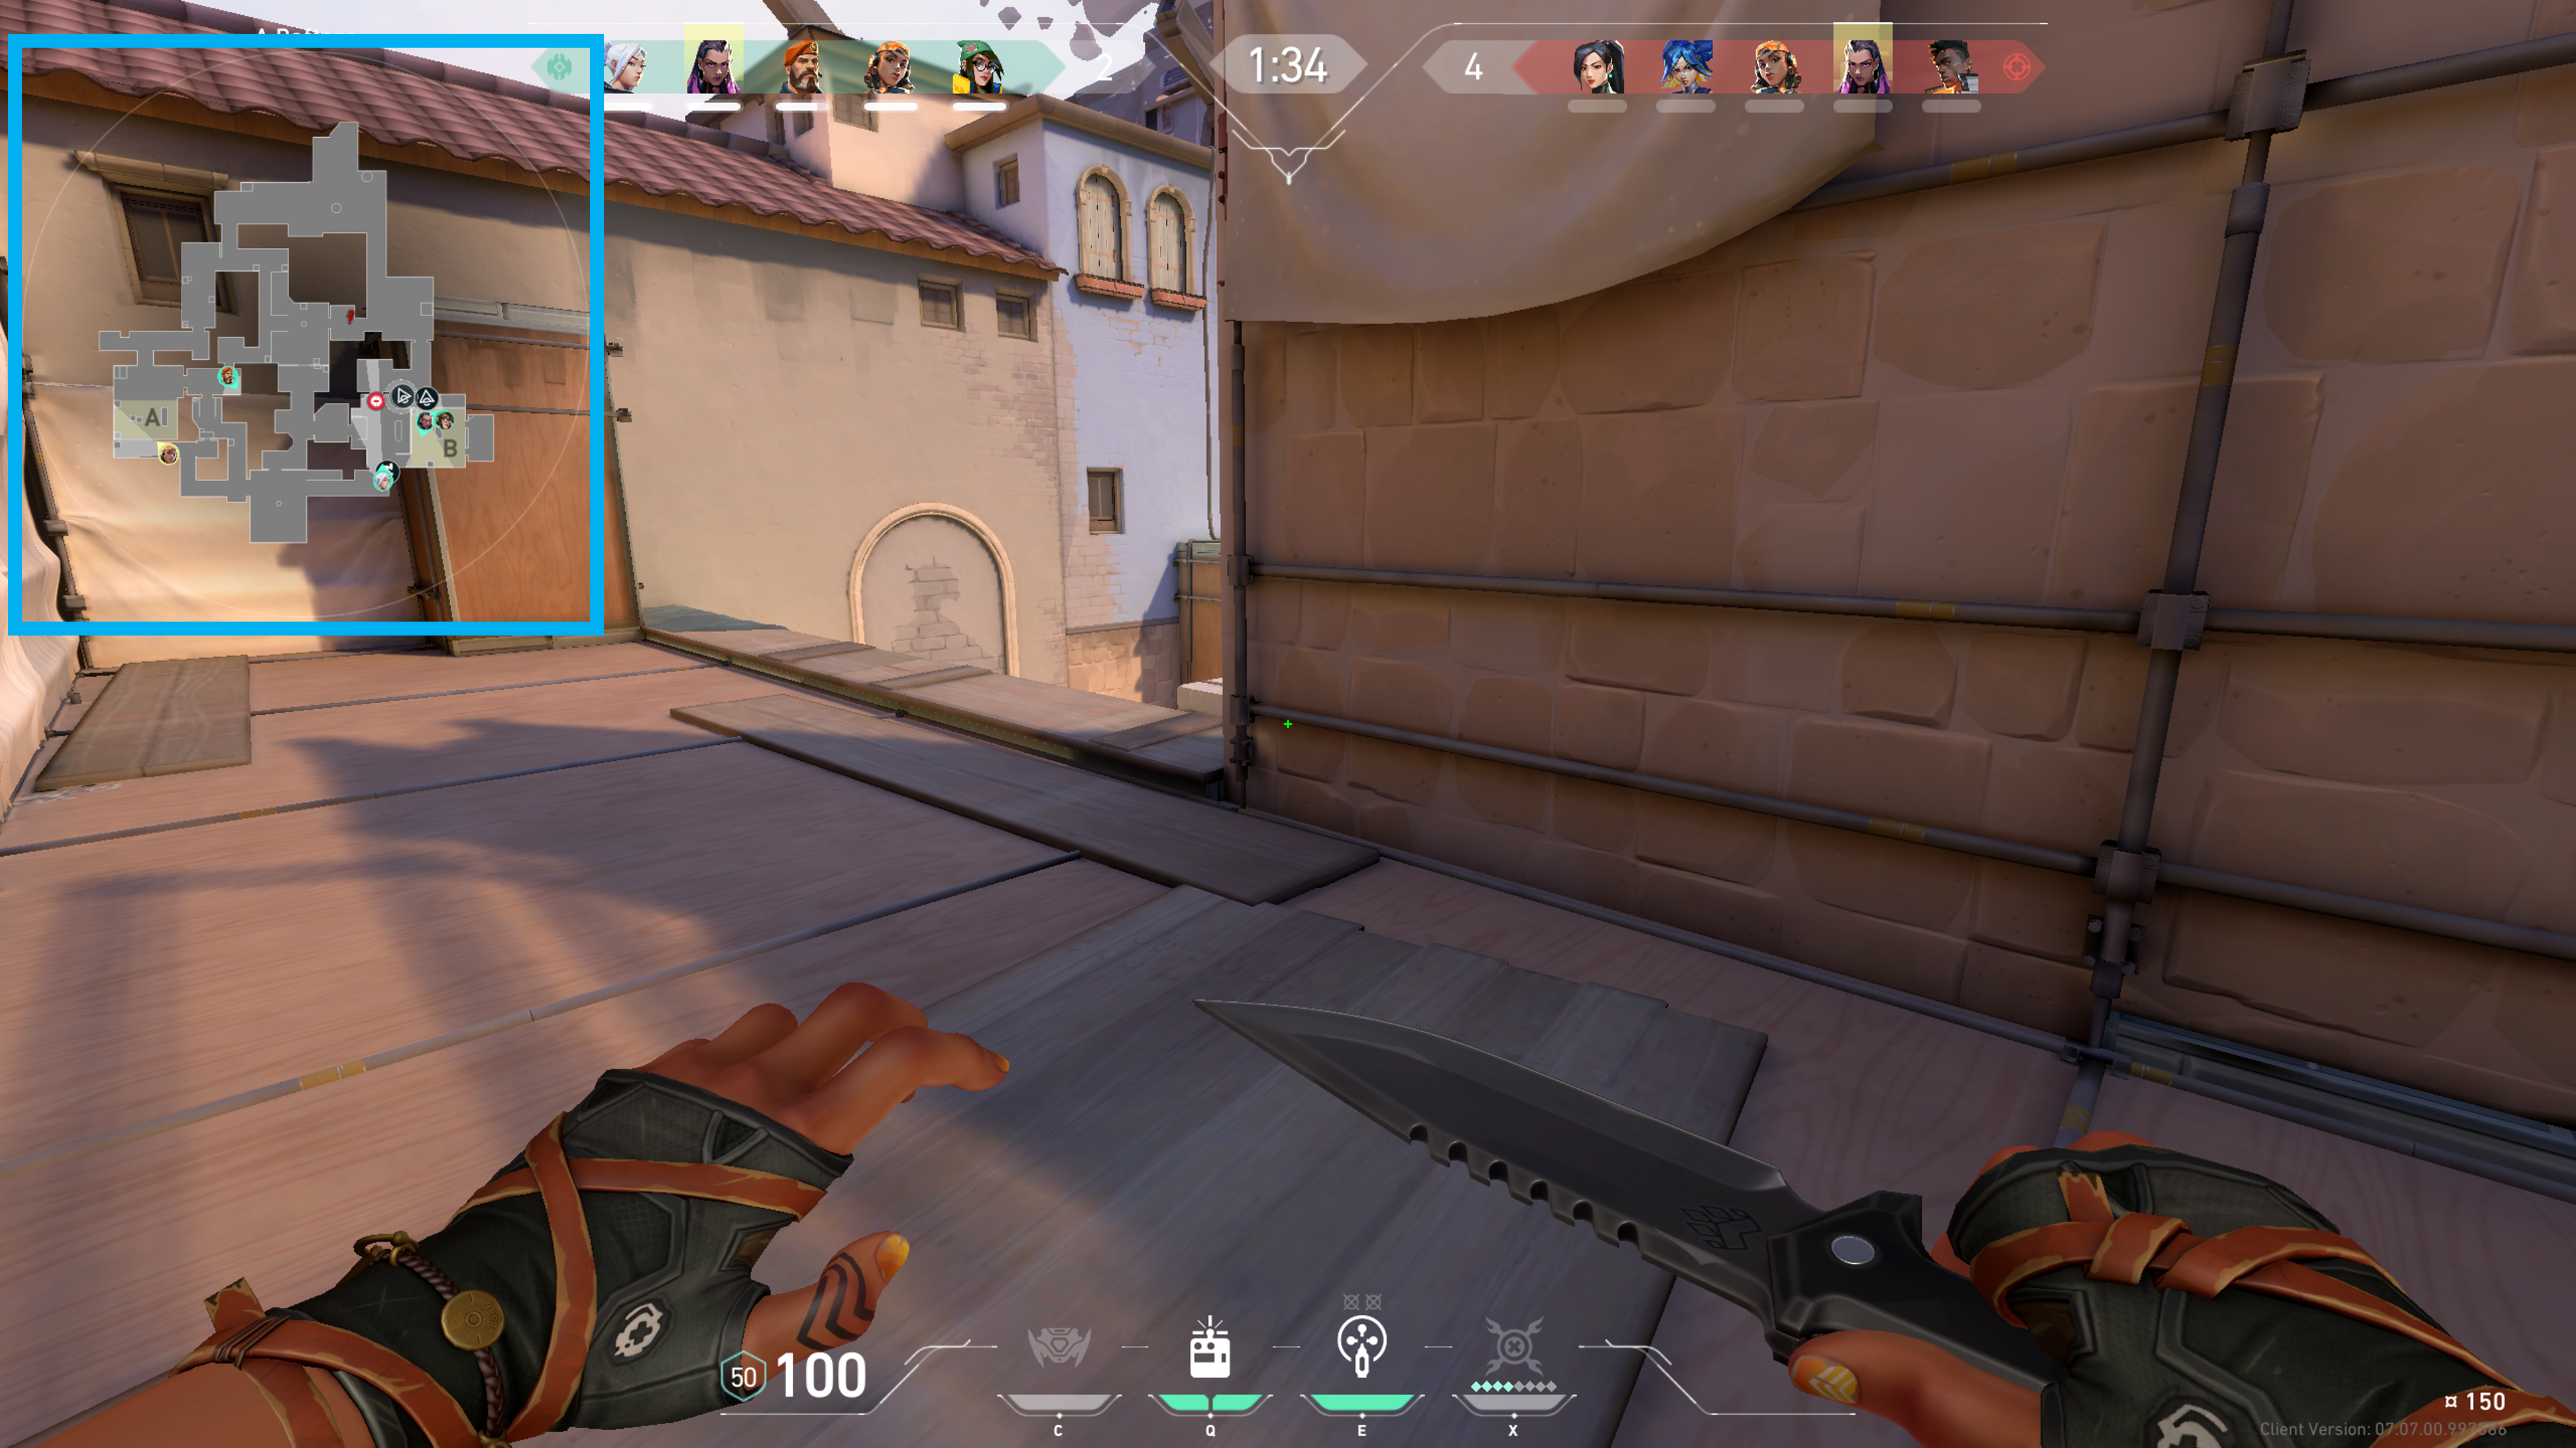
\includegraphics[width=0.95\linewidth]{images/02-ingame-minimap}
	\caption[In-game screenshot of Valorant]{In-game screenshot of Valorant with a marker on the 
	minimap.}
	\label{fig:intro:ingame}
\end{figure}

\autoref{fig:intro:ingame} shows an in-game screen of Valorant from players perspective. Most 
important for this project is the blue marked part in the upper left corner. This is the minimap that 
gives an overview of the map\footnote{In that case it is the map "Ascent".} and where teammates or 
agent abilities are placed. In image~\ref{fig:intro:minimap} a zoomed version of this minimap can be 
seen. The gray area is an illustration of the map with the most distinctive points. Normally it is used 
for orientation. Furthermore on the minimap the teammates can be found, two of them are marked 
with a blue square. All five agents in that image are in the same team and on defender side. The side 
can be identified by the color "green" that surrounds the characters\footnote{Attackers would be 
pictured in red.}.  Except for the agent on the far left: that color is yellow, but that means that this is 
the agent whose perspective the screenshot is from, but he is also a defender. The item marked in 
yellow is an ability of an agent from the defender team. The red point marked with pink is an ability 
from an attacker/enemy. The two areas named "A" and "B" are the plant spots where the bomb can 
be placed as mentioned before.

\begin{figure}
	\centering
	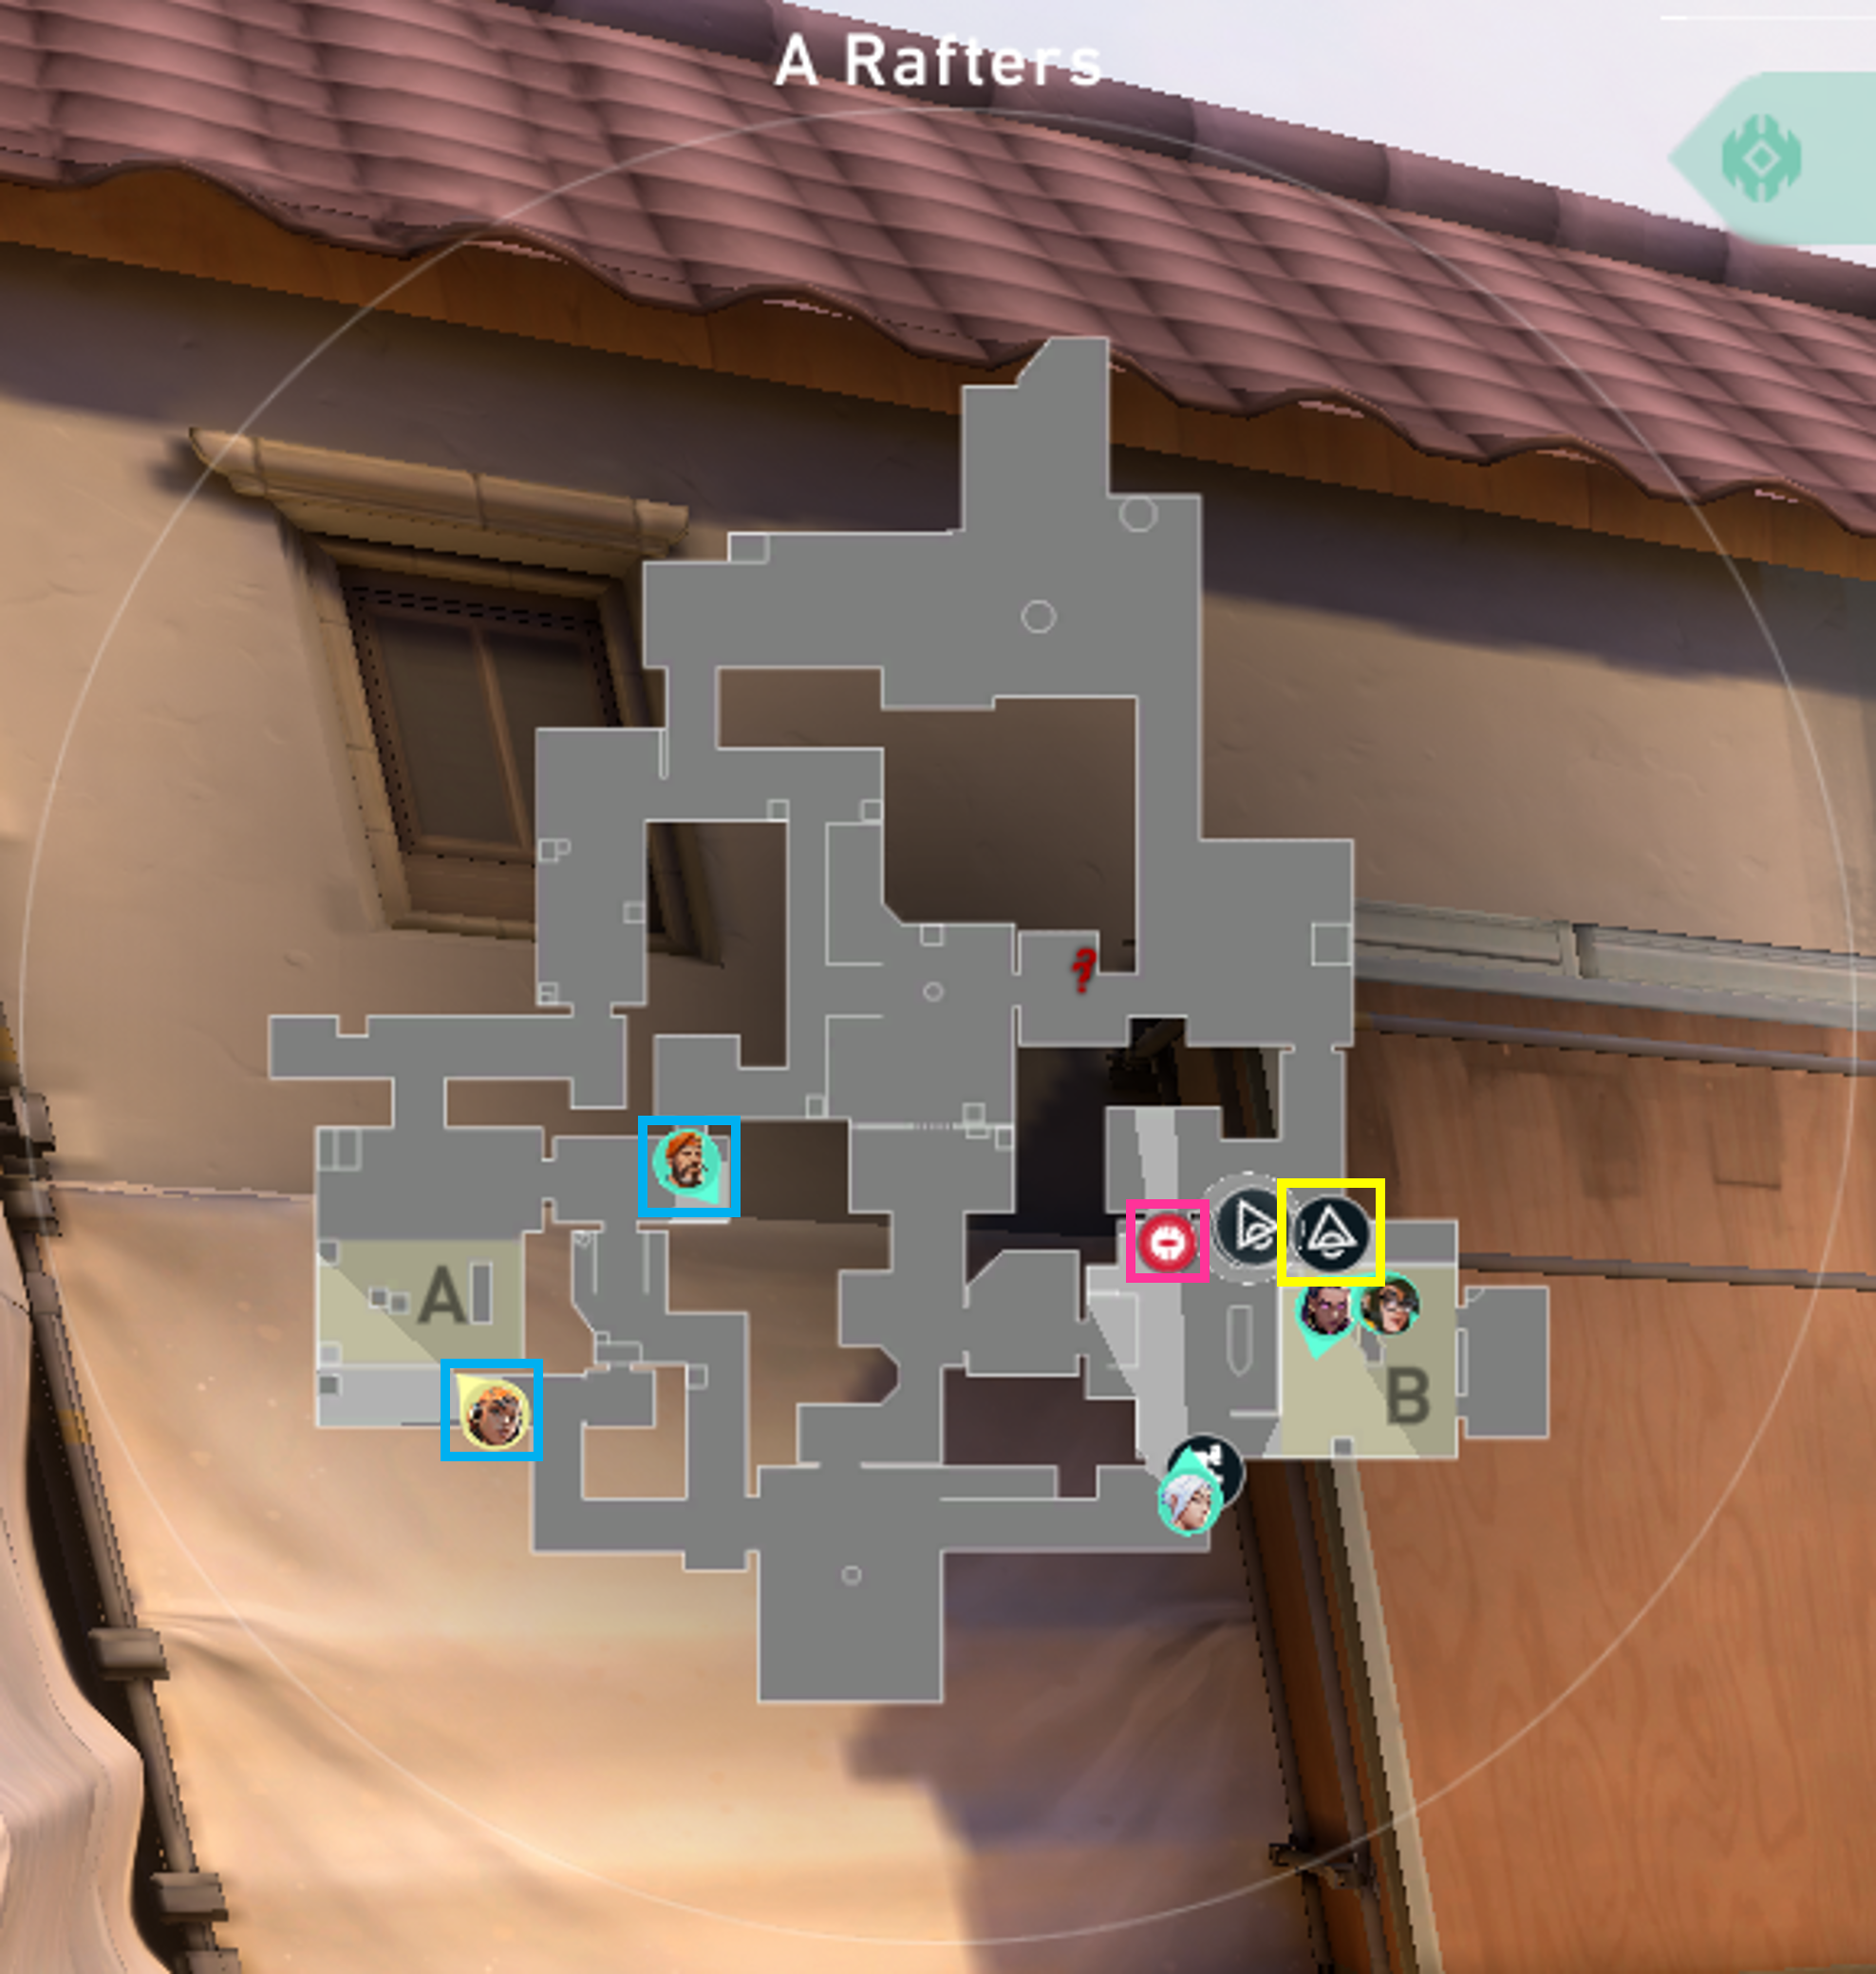
\includegraphics[width=0.86\linewidth]{images/04-minimap-marker}
	\caption[Valorant minimap]{Valorant minimap with teammates (blue), team abilities (yellow) and 
	enemy ability (pink).}
	\label{fig:intro:minimap}
\end{figure}


\section{Related Work}\label{sec:intro:relatedWork}

\chapter{Application}\label{chpt:application}
\glsresetall

\section{Concept}\label{sec:app:concept}

\section{Data}\label{sec:app:data}

\section{YOLOv5}\label{sec:app:yolov5}

\section{Implementation}\label{sec:app:impl}

\section{Dataset}\label{sec:app:dataset}

\section{Summary}\label{sec:app:summary}

\chapter{Evaluation}\label{chpt:evaluation}
\glsresetall

\section{Experiments}\label{sec:eval:experiments}

\section{Results}\label{sec:eval:results}

\section{Discussion}\label{sec:eval:discussion}

\chapter{Conclusion and Future Work}\label{chpt:conclusion+future}
\glsresetall

Finally a summary is provided and further ideas for project extension are given in the 
section~\ref{sec:future}.

\section{Conclusion}\label{sec:conclusion}

In this project a concept for an application was successfully developed and implemented. The 
application transforms a recording of the video game Valorant into a new representation that gives 
a better overview of the rounds for players and trainers and helps them to improve their skills.

The realization of this concept includes acquiring of data as well as the pre-pro\-ces\-sing of it with 
the objective to build a dataset. As training framework YOLOv5 from Ultralytics was chosen. In order 
to complete the training task it was necessary to get used to YOLOv5 and miscellaneous concepts in 
the field of the training of a neural network. Furthermore a script was implemented to transform the 
output of the neural network into an image, so that it is better understandable.

Challenging was to get enough labeled data because the preparation of it is very time consuming. 
Another problem is the limited hardware performance on private computers. These cause long 
training times and low performance networks have to be used which affect the results. But all in all 
satisfying results could be achieved.

\section{Future Work}\label{sec:future}

In following projects the learning task can be extended onto the detection of individual agents and 
abilities. With that information more helpful output formats can be developed. Additionally other 
learning techniques can be applied like the usage of time series processing algorithms. 
They could use available time information from videos for better detection. Furthermore it would be 
possible to use the output of neural networks, like that from this project, as input of other pattern 
recognition algorithms. These could be used to evaluate the gameplay in an advanced way.


\appendix
\chapter{Additions to the application}\label{chpt:applicationAdditions}
\glsresetall

\section{Architecture of Yolov5}\label{sec:aa:archyolov5}

\begin{figure}[H]
	\centering
	\includegraphics[width=1.0\linewidth]{images/a01-arch-yolov5}
	\caption[Architecture of YOLOv5.]{Architecture of YOLOv5~\cite{archYolov5}.}
	\label{fig:aa:archyolov5}
\end{figure}


\chapter{Additions to the evaluation}\label{chpt:evaluationAdditions}
\glsresetall

\section{Training metrics}\label{sec:ea:trainingMetrics}

\begin{longtable}{p{0.03\textwidth}p{0.17\textwidth}p{0.03\textwidth}p{0.14\textwidth}p{0.03\textwidth}S[table-format=1.3]S[table-format=1.3]S[table-format=1.3]S[table-format=1.4]}
	\caption[Overview of all metric results.]{Overview of metric results for different training tasks and data splits.}\label{tab:ea:metricResults} \\
	\toprule
	&  \multicolumn{1}{c}{Training task} &&  \multicolumn{1}{c}{Epoch} && \multicolumn{1}{c}{$P$} & \multicolumn{1}{c}{$R$} & \multicolumn{1}{c}{$mAP_{50}$} & \multicolumn{1}{c}{$mAP_{50-95}$} \\
	\midrule
	\endfirsthead
	%
	\toprule
	&  \multicolumn{1}{c}{Training task} &&  \multicolumn{1}{c}{Epoch} && \multicolumn{1}{c}{$P$} & \multicolumn{1}{c}{$R$} & \multicolumn{1}{c}{$mAP_{50}$} & \multicolumn{1}{c}{$mAP_{50-95}$} \\
	\midrule
	\endhead
	%
	\multicolumn{9}{l}{\bfseries{Model 1, Validation data}} \\[7pt]
	%
	&  \multicolumn{1}{c}{\textsc{train}} &&  \multicolumn{1}{c}{\textsc{last}} && 0.975 & 0.982 & 0.988 & 0.675 \\[5pt]
	&  \multicolumn{1}{c}{\textsc{train}} &&  \multicolumn{1}{c}{\textsc{best}} && 0.982 & 0.974 & 0.988 & 0.664 \\[9pt]
	%
	&  \multicolumn{1}{c}{\textsc{finetune}} &&  \multicolumn{1}{c}{\textsc{last}} && 0.994 & 0.988 & 0.995 & 0.823 \\[5pt]
	&  \multicolumn{1}{c}{\textsc{finetune}} &&  \multicolumn{1}{c}{\textsc{best}} && 0.993 & 0.988 & 0.995 & 0.825 \\[7pt]
	%
	\multicolumn{9}{l}{\bfseries{Model 1, Test data}} \\[7pt]
	%
	&  \multicolumn{1}{c}{\textsc{train}} &&  \multicolumn{1}{c}{\textsc{last}} && 0.973 & 0.982 & 0.99  & 0.668 \\[5pt]
	&  \multicolumn{1}{c}{\textsc{train}} &&  \multicolumn{1}{c}{\textsc{best}} && 0.974 & 0.977 & 0.991 & 0.661 \\[9pt]
	%
	&  \multicolumn{1}{c}{\textsc{finetune}} &&  \multicolumn{1}{c}{\textsc{0}} && 0.254 & 0.977 & 0.254 & 0.0684 \\[5pt]
	&  \multicolumn{1}{c}{\textsc{finetune}} &&  \multicolumn{1}{c}{\textsc{5}} && 0.934 & 0.956 & 0.981 & 0.741  \\[5pt]
	&  \multicolumn{1}{c}{\textsc{finetune}} &&  \multicolumn{1}{c}{\textsc{10}} && 0.982 & 0.985 & 0.991 & 0.794  \\[5pt]
	&  \multicolumn{1}{c}{\textsc{finetune}} &&  \multicolumn{1}{c}{\textsc{15}} && 0.983 & 0.983 & 0.992 & 0.807  \\[5pt]
	&  \multicolumn{1}{c}{\textsc{finetune}} &&  \multicolumn{1}{c}{\textsc{20}} && 0.98  & 0.986 & 0.991 & 0.81   \\[5pt]
	&  \multicolumn{1}{c}{\textsc{finetune}} &&  \multicolumn{1}{c}{\textsc{25}} && 0.98  & 0.988 & 0.992 & 0.813  \\[5pt]
	&  \multicolumn{1}{c}{\textsc{finetune}} &&  \multicolumn{1}{c}{\textsc{30}} && 0.982 & 0.985 & 0.992 & 0.813  \\[5pt]
	&  \multicolumn{1}{c}{\textsc{finetune}} &&  \multicolumn{1}{c}{\textsc{35}} && 0.982 & 0.986 & 0.993 & 0.815  \\[5pt]
	&  \multicolumn{1}{c}{\textsc{finetune}} &&  \multicolumn{1}{c}{\textsc{40}} && 0.979 & 0.99  & 0.993 & 0.816  \\[5pt]
	&  \multicolumn{1}{c}{\textsc{finetune}} &&  \multicolumn{1}{c}{\textsc{45}} && 0.979 & 0.991 & 0.993 & 0.815  \\[5pt]
	&  \multicolumn{1}{c}{\textsc{finetune}} &&  \multicolumn{1}{c}{\textsc{50}} && 0.979 & 0.992 & 0.994 & 0.816  \\[5pt]
	&  \multicolumn{1}{c}{\textsc{finetune}} &&  \multicolumn{1}{c}{\textsc{55}} && 0.981 & 0.991 & 0.994 & 0.811  \\[5pt]
	&  \multicolumn{1}{c}{\textsc{finetune}} &&  \multicolumn{1}{c}{\textsc{60}} && 0.979 & 0.992 & 0.994 & 0.817  \\[5pt]
	&  \multicolumn{1}{c}{\textsc{finetune}} &&  \multicolumn{1}{c}{\textsc{65}} && 0.979 & 0.99  & 0.994 & 0.82   \\[5pt]
	&  \multicolumn{1}{c}{\textsc{finetune}} &&  \multicolumn{1}{c}{\textsc{70}} && 0.981 & 0.992 & 0.994 & 0.815  \\[5pt]
	&  \multicolumn{1}{c}{\textsc{finetune}} &&  \multicolumn{1}{c}{\textsc{75}} && 0.98  & 0.992 & 0.994 & 0.815  \\[5pt]
	&  \multicolumn{1}{c}{\textsc{finetune}} &&  \multicolumn{1}{c}{\textsc{80}} && 0.981 & 0.99  & 0.994 & 0.817  \\[5pt]
	&  \multicolumn{1}{c}{\textsc{finetune}} &&  \multicolumn{1}{c}{\textsc{85}} && 0.981 & 0.991 & 0.994 & 0.817  \\[5pt]
	&  \multicolumn{1}{c}{\textsc{finetune}} &&  \multicolumn{1}{c}{\textsc{90}} && 0.98  & 0.991 & 0.994 & 0.82   \\[5pt]
	&  \multicolumn{1}{c}{\textsc{finetune}} &&  \multicolumn{1}{c}{\textsc{95}} && 0.981 & 0.991 & 0.994 & 0.82   \\[5pt]
	%
	&  \multicolumn{1}{c}{\textsc{finetune}} &&  \multicolumn{1}{c}{\textsc{last}} && 0.98  & 0.992 & 0.994 & 0.819 \\[5pt]
	&  \multicolumn{1}{c}{\textsc{finetune}} &&  \multicolumn{1}{c}{\textsc{best}} && 0.981 & 0.991 & 0.994 & 0.819 \\[7pt]
	%
	\multicolumn{9}{l}{\bfseries{Model 2, Validation data}} \\[7pt]
	%
	&  \multicolumn{1}{c}{\textsc{train}} &&  \multicolumn{1}{c}{\textsc{last}} && 0.987 & 0.991 & 0.993 & 0.68 \\[5pt]
	&  \multicolumn{1}{c}{\textsc{train}} &&  \multicolumn{1}{c}{\textsc{best}} && 0.985 & 0.992 & 0.993 & 0.682 \\[7pt]
	%
	\multicolumn{9}{l}{\bfseries{Model 2, Test data}} \\[7pt]
	%
	&  \multicolumn{1}{c}{\textsc{train}} &&  \multicolumn{1}{c}{\textsc{last}} &&  0.984 & 0.986 & 0.991 & 0.673 \\[5pt]
	&  \multicolumn{1}{c}{\textsc{train}} &&  \multicolumn{1}{c}{\textsc{best}} &&  0.983 & 0.99  & 0.991 & 0.676 \\
	%
	\bottomrule
\end{longtable}

\newpage

\section{Inference results}\label{sec:ea:inferenceResults}

\begin{figure}[H]
	\centering
	\includegraphics[width=0.8\linewidth]{images/a02-detect}
	\caption[Detected bounding boxes.]{Detected bounding boxes for a not trained image from the map "Ascent".}
	\label{fig:ea:outDetect}
\end{figure}

\begin{figure}[H]
	\centering
	\includegraphics[width=0.95\linewidth]{images/a03-att-output}
	\caption[Output representation as map for attacker.]{Output representation as map, summarizing all positions 
		of attacker agents during one round on the map "Haven".}
	\label{fig:ea:outputAtt}
\end{figure}

\begin{figure}[H]
	\centering
	\includegraphics[width=0.95\linewidth]{images/a04-comb-output}
	\caption[Output representation as map.]{Output representation as map, summarizing all positions 
		of defender and attacker agents during one round on the map "Haven".}
	\label{fig:ea:outputComb}
\end{figure}

\backmatter
\printglossaries

\clearpage
\phantomsection
\addcontentsline{toc}{chapter}{\listfigurename}
\listoffigures

\clearpage
\phantomsection
\addcontentsline{toc}{chapter}{\listtablename}
\listoftables

%\renewcommand\lstlistlistingname{Codeverzeichnis}
%\clearpage
%\phantomsection
%\addcontentsline{toc}{chapter}{\lstlistlistingname}
%\lstlistoflistings
\printbibliography

\clearpage
\thispagestyle{empty}

Name: \fullname \hfill Matriculation number: \matnr \vspace{2cm}

\minisec{Statement}

I declare that I have independently written the thesis and have not used any sources or aids other 
than those specified.\vspace{2cm}

Ulm, \dotfill

\hspace{10cm} {\footnotesize \fullname}
\end{document}
